\documentclass[11pt]{article}

\usepackage{lineno}

\usepackage{tikz}
\usetikzlibrary{shapes, arrows.meta, positioning}

\usepackage{makecell}
\usepackage{charter}
%\usepackage{euler}
\usepackage{inconsolata}
\usepackage{xcolor}
\usepackage[alternateNonterms]{ottalt}
\usepackage{amsmath}
\usepackage{geometry}
\usepackage{graphicx}

% \usepackage{bm} % bold tt font in math mode

\geometry{margin=1in}

\inputott{formalism-commands}

\renewcommand{\ottkw}[1]{\textbf{\texttt{#1}}}

%\renewcommand{\ottcom}[1]{\textit{#1}}

%% \newcommand{\ottnt}[1]{\ensuremath{mathit{#1}}}
%% \newcommand{\ottmv}[1]{\ensuremath{\mathit{#1}}}
%% \newcommand{\ottkw}[1]{\ensuremath{\mathbf{#1}}}
%% \newcommand{\ottcom}[1]{{#1}}
%% \newcommand{\ottsym}[1]{{#1}}

\begin{document}

\author{Matthew A. Hammer}
\title{The Adapton Recipe
  \\
  \small The Essence of Demanded Computation Graphs
}

\maketitle

\linenumbers

\section{Introduction}

A computer program has the \emph{potential} to be \textbf{incremental} if
rerunning it on similar inputs results in similar steps, and similar
outputs.
%
A \emph{fully-realized} incremental program is one where the observed
behavior is consistent with a simple, redundancy-having computer program,
but where the redundant work for similar steps is
avoided, somehow (often using some space), making it more efficient to compute in time.

The space consumed by an incremental program can store anything useful
to save time later, and often employs techniques that involve
memoization (function caching) and/or dynamic dependency graphs.
%
Adapton gives a recipe for \textbf{\emph{general-purpose incremental
  computation}} that employs its own variation of these techniques,
and hides them under a special set of programming-language-level
abstractions.
%
\begin{itemize}
\item ``\textbf{general-purpose}'' here means we care about programs
  with \emph{general recursion, over general-purpose data structures}
  with or without mutation and cycles (as opposed to a more restricted
  domain-specific language), and
  
\item ``\textbf{incremental}'' here means two complementary things at once:
  \begin {itemize}

  \item that the \textbf{program's input mutates incrementally} by the
    ambient editor program or user, in arbitrary change batches (more than one, generally), and 
    
  \item that the \textbf{program's output is demanded incrementally}
    by that ambient editor.
  \end{itemize}
\end{itemize}

\noindent
Adapton's recipe is a PL design and implementation recipe, best
applied by a team doing both, with full control over both.
%
It affects the programming model exposed to the programmer, as well as
the runtime system used by the language's implementation.
%
The recipe maps a purely functional fragment of this team's PL into
another PL fragment that is both incremental and stateful, enriching
the original (subset of the) source PL with read and write operations
on global state.


\begin{center}
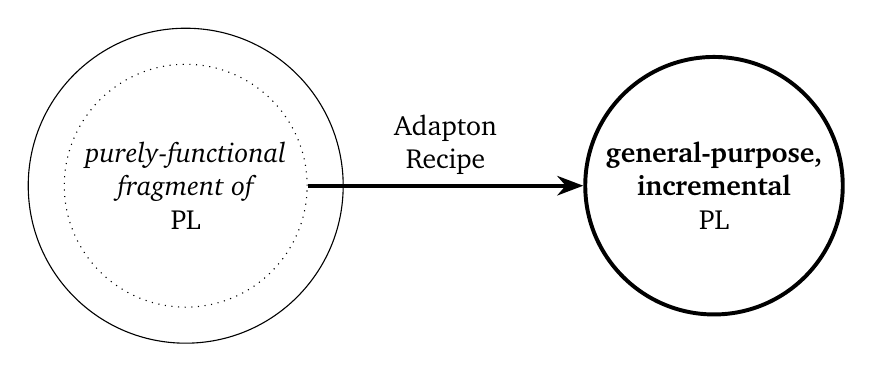
\begin{tikzpicture}[node distance=3.5cm, every node/.style={draw, align=center}]

  % Left outer blob
  \node (outerblob) [circle, minimum size=4cm] {};
  
  % Left inner blob
  \node (innerblob) [circle, minimum size=2.5cm, dotted] at (outerblob.center) {\it purely-functional\\\it fragment of\\ PL};

  % Right blob
  \node (rightblob) [circle, minimum size=2.5cm, right=of innerblob, line width=0.5mm] {\bf general-purpose,\\\bf incremental\\ PL};

  % Arrow with text
  \draw[->,  line width=0.5mm, >=Stealth] (innerblob) -- node[midway, above, draw=none] {Adapton\\Recipe} (rightblob);

\end{tikzpicture}
\end{center}

\noindent
By employing these special primitives, the program expresses dependencies
between inputs and outputs (reading the former and writing the later),
and Adapton hides the complexity of representing and maintaining these
dynamic dependencies.

Behind the scenes, Adapton's recipe provides the demanded computation graph (DCG),
including the semantics for the graph components'
memoization and change propagation\footnote{
In a sense, Adapton enriches the existing (CBV or CBN)
\emph{evaluation strategy} of a PL with an additional dimension of
evaluation that requires a persistent a graph representation of the
program's past behavior.
%
In this presentation of the recipe, we focus on a CBV host language.
%
Past presentations used call-by-push-value (CBPV) which avoids the
choice between CBV and CBN by subsuming both; however, a CBPV
presentation can be confusing for newcomers, so we use CBV here.
}.

In this graph-based strategy, there's an ambient memory (global state)
for communicating values between different points of incremental
space-time, based on symbolic names whose definitions persist across
distinct incremental runs.
%
These symbols name the program's individual steps and datums in a way
that identifies their ``change positions'' symbolically.
%
This level of indirection turns out to be critical for efficient
incremental responses to changes.

Adapton's notion of ``ambient memory'' (and the graphs that implement
it) permit computations to be \emph{impure} in at least two practical
ways:

\begin{itemize}

\item \textbf{Reading} from incrementally-changing global state, such as state controlled directly by interactive user input that edits it.
  
\item \textbf{Writing} to incrementally-changing global state, including intermediate results and the final output of the computation.

\end{itemize}

Adapton prescribes a general way to augment a functional
programming language with primitives to handle these read and write effects.


\section{Symbols}


This Adapton recipe uses the notion of ``symbols.'' A symbol is a
unique identifier, determined dynamically by a running program, or fed
as part of its input, or some combination of those two methods.
%
When used to name something, like a specific datum or sub-computation,
the incremental program also implicitly says when and where to reuse
it later, as the program re-executes incrementally.

\ottgrammartabular{
  \otts
}

Each symbol $\ottnt{s}$ is made of one or more literals,
combined with binary composition operators.
%
The details of these literal symbols (numbers, strings, etc) and
binary composition operators is inconsequential to the rest of the
Adapton recipe.  Any conventions that make sense for the ambient host PL will work.

Here, we assume three binary composition forms that get overloaded: the
dot operator usually reserved for field access, and the minus operator
usually reserved for arithmetic, and the application form usually reserved for function calls.
%
We overload these forms to construct symbol trees.
%
The intention of minus and dot here are to mimick common composit
names in UNIX, where dashes and dots are common word separators.
%
We use the application form to indicate sub-spaces and sub-moments.

\section{Symbolic Space and Time.}

Each program or library that uses the Extended Adapton Recipe (EAR)
defines a system of symbolic names for space and time.
The details of this system are program/library-specific, and the
design of EAR itself affords a chance to compose distinct systems to
create larger ones.
Essentially, the chance to compose distinct systems stems from the choice of moments
and space to each be \emph{nestable} (or \emph{fractal}) in nature.

\ottgrammartabular{
  \ottSpace
  \\
  \ottMoment
  \\
  \ottp
  \\
  \ottpp
  \\
  \ottd
}

Programs using EAR have control over space and time in ways
that ordinary programs do not.
%
One aspect of this control is the distinction between
\emph{space-time} and \emph{time-space} regions of the store, which are complementary in
the recipe.
%
The storage used by the program distinguishes these regions as follows.
%
Space-time ($[[d = st]]$) holds data that ``is'' part of a moment.
By contrast,
time-space ($[[d = ts]]$) holds data that is ``becoming'' part of a moment.

When the program navigates time, this data that is ``becoming'' part
of the target moment transitions atomically into what ``is'' at that
target moment where the program arrives.
%
See Sections~\ref{sec:refsem-navigation} and~\ref{sec:refsem-undelay}.

\section{Programs}

The Adapton recipe we present here assumes a CBV host language, with a
pre-existing model of common language features, such as recursive data
types, recursive functions, pattern matching, and other details.
%
To this host language, the recipe adds a handful of special value
forms and special expression forms.

\paragraph{Values.}

\ottgrammartabular{
  \ottv
}

\paragraph{Role of thunks in the recipe.}
In contrast to earlier CBPV-based presentations that fused all thunks
with the ambient global state (PLDI 2014 and OOPSLA 2015), here we
assume ordinary thunks exist in the host language already and we treat
them as a distinct, ordinary value type.
%
Because they are central to the special new forms, we illustrate their
(pure) dynamics in detail, though again this dynamics is the ordinary one.


\paragraph{Expressions.}

We begin by assuming usual CBV expression forms, and thunks.
%
To these forms, the Adapton recipe also adds expression forms that
affect the ambient graph: \textbf{put}, \textbf{get}, \textbf{force}
and \textbf{do}, each using the new value forms of symbols or
pointers, or both.  The functions \textbf{here} and \textbf{now} would
practically be exposed with a library, but we include them here for
illustration.

\ottgrammartabular{
  \otte
}

\ottgrammartabular{
  \ottC
  \\
  \ottCxtVerb
  \\
  \ottCxtDim
}  

We introduce some syntactic sugar.

\paragraph{Do-at notation.}

The ``do-at'' notation is shorthand for the common programming idiom
of writing a thunk to the graph within a space (here,~$[[e1]]$) and then
immediately forcing it's evaluation (the body~$[[e2]]$):

\[
\begin{array}{lcl}
  [[do @e1 { e2 }]]
  &\equiv&
  [[let x = put(e1, thunk(e2)) in]]
  \\
  &&[[force(x)]]
\end{array}
\]

\paragraph{Do-at-within notation.}
Another common variation of this shorthand does the thunk within a
certain subspace:

\[
\begin{array}{lcl}
  [[do @e1 within e2 { e3 }]]
  &\equiv&
  [[let x = put(e1, thunk(do within space (e2){e3})) in]]
  \\
  &&[[force(x)]]
\end{array}
\]

\noindent
Sometimes, it can be preferable (and simpler) to reuse the same symbol
as the thunk-naming symbol to name this subspace:

\[
\begin{array}{lcl}
  [[do @within e1 { e2 }]]
  &\equiv&
  [[let x = put(e1, thunk(do within space (e1){e2})) in]]
  \\
  &&[[force(x)]]
\end{array}
\]

\section{Reference Dynamics}

Programs here have a reference dynamics and an incremental dynamics.

While the incremental dynamics describes dependence graphs, the
reference dynamics describes a more limited flavor of caching that is
intolerant of most effects (except for the effect of updating the
cache with otherwise-pure computation results).

The role of the reference dynamics is to capture this limited form of
caching that lacks dependence graphs, giving a basis for comparison
for the incremental dynamics that requires and uses dependence graphs
throughout.

\begin{tabular}{cc}
  \\[0mm]
\begin{minipage}{0.42\textwidth}
\ottgrammartabular{
  \ottStore
}
\end{minipage}
&
\begin{minipage}{0.43\textwidth}
\ottgrammartabular{
  \ottcell
}
\end{minipage}
\end{tabular}

\[
\begin{array}{lc}
\scalebox{1.5}{\boxed{
  [[Store1; Path; Moment; Space |- e !! Store2; v]]
}}
&
\begin{array}{p{4in}}
  ``
  Under store~$[[Store1]]$,
  path~$[[Path]]$,
  space~$[[Space]]$,
  and
  moment~$[[Moment]]$,\\
  \hspace{3mm}~expression~$[[e]]$ evaluates fully,\\
  \hspace{6mm}~resulting in store~$[[Store2]]$ and value~$[[v]]$.
  ''
\end{array}
\end{array}
\]


\subsection{Pure thunks.}

Thunk values that are not stored are forced in the usual way:

\[
\drule{EXXthunk}
\drule{EXXforceThunk}
\]

\subsection{Symbol expressions.}

Symbols are values:

\[
\drule{EXXsym}
\]

Some expressions produce symbol trees:

\[
\drule{EXXsymMinus}
\drule{EXXsymDot}
\drule{EXXsymApp}
\]

\subsection{Put and get.}

Put and get operations give write and read access to the global store.

\[
\begin{array}{cc}
  \drule{EXXputImmediate}
  &
  \drule{EXXgetNonThunk}
  \\[2mm]
  \drule{EXXputDelay}
  &
  \drule{EXXgetThunk}
\end{array}
\]

There are two temporal cases for putting a value into the store (immediate in space-time, or delayed in time-space).
%
Each value put into the store can either be a thunk or a non-thunk value.
For a thunk, the store update syntax $[[Store{pp |-> (Space, v)}]]$
means that $[[v = thunk(e)]]$ for some expression~$[[e]]$,
and this update is defined as $[[Store{pp |-> Thunk(Space, e, empty)}]]$.
Alternatively, when $[[v /= thunk(e)]]$, 
the update ignores the space~$[[Space]]$ and is defined instead as $[[Store{pp |-> NonThunk v}]]$.

For the two \texttt{get} rules, the store access $[[Store((Space2, Moment) ^ st) = cell]]$ compares the current moment~$[[Moment]]$ to those written at the given space~$[[Space2]]$, choosing the ``latest'' cell whose moment is equal to or earlier than~$[[Moment]]$, if it exists.
It is not defined when no such moment exists.
There are two cases, depending on whether~$[[cell]]$ is a non-thunk value, or a thunk cell.
For the latter, the operation returns a pair that includes the space value used by the thunk (note that $[[Space1]]$, $[[Space2]]$ and $[[Space0]]$ can all be distinct).

\subsection{Navigating space-time.}
\label{sec:refsem-navigation}

\[
\begin{array}[t]{p{0.731in}|c|c}
  & \textbf{Space} & \textbf{Time}
  \\[2mm]
  \hline
  &&
  \\[2mm]
  \begin{tabular}[l]{l}\texttt{here},\\\texttt{now}\end{tabular}
  & \drule{EXXhere}
  & \drule{EXXnow}
  \\[2mm]
  \hline
  &&
  \\[2mm]
  
  \texttt{goto}
  &
  \drule{EXXgotoSpace}
  &
  \drule{EXXgotoMoment}
  \\[2mm]
  \hline
  &&
  \\[2mm]

  \texttt{within}
  &
  \drule{EXXwithinSpace}
  &
  \drule{EXXwithinMoment}
\end{array}
\]

\subsection{Navigating time: Undelay}
\label{sec:refsem-undelay}

\begin{mathpar}
\drule{undelayXXempty}
\drule{undelayXXbinary}
\drule{undelayXXmoment}
\drule{undelayXXskipMoment}
\drule{undelayXXskipSpace}
\end{mathpar}

\subsection{Forcing a thunk pointer.}

 \begin{mathpar}
\drule{EXXemptyForce}
\drule{EXXreuseForce}
\drule{EXXredoForce}
\end{mathpar}

\subsection{Aligned stores}

\[
\begin{array}{ll}
\boxed{
  [[Store1 <= Store2]]
}
&
\text{``Store $[[Store2]]$ is an aligned extension of store~$[[Store1]]$''}
\end{array}
\]

\begin{mathpar}
  \drule{AXXempty}
  \drule{AXXbinary}
  \drule{AXXcell}
  \drule{AXXcache}
\end{mathpar}
\[
\drule{AXXequiv}  
\]

\[
\begin{array}{ll}
\boxed{
  [[Store1 </= Store2]]
}
&
\text{``Store $[[Store2]]$ is \textbf{not} an aligned extension of store~$[[Store1]]$''}
\end{array}
\]

\begin{mathpar}
  \drule{NAXXfocus}
  \drule{NAXXchanged}
  \drule{NAXXforgot}
\end{mathpar}

\section{Graphs}

A graph $[[Graph]]$ consists of named nodes with special payload and edge
structure.
  
\ottgrammartabular{
  \ottGraph
}

\ottgrammartabular{
  \ottppp
  \\
  \ottnode
  \\
  \ottcache
  \\
  \ottt
  \\
  \ottedge
  \\
  \ottA
  \\
  \ottb
}

\paragraph{Nodes.}

\paragraph{Edges.}

\paragraph{Well-formed graphs.}


To ensure that incremental evaluation always produces results
consistent with from-scratch evaluation (a form of ``incremental
correctness''), graphs must remain \textbf{well-formed}, an invariant
formally required by the dynamics.

A graph is well-formed when each evaluated node has a cached result
from some earlier run on a well-formed graph.
%
That earlier run can be very out-dated with respect to the current graph.
%
In those cases, an additional aspect of the graph being well-formed
also insists on the status of an edge be dirty whenever its truly
outdated, or depends on some edge that is, transitively.
%
The dirty status can be overly-conservative, but it must hold
transitively, in every case.

More operationally, each write effect to a graph node also traverses
the dependencies of immediately affected edges, whenever the new value
differs from the originally-observed one on such an edge.
%
A transitively affected node is either a directly affected node
itself, a node that directly forces a directly affected node, or one
that transitively forces it.


\section{Graph Dynamics}

\[
\begin{array}{lc}
  {\scalebox{1.5}{
  \boxed{[[Graph1; Path; Moment; m; Space |- e !! Graph2; t; v]]}}}
&
\begin{array}{p{4in}}
  ``
  Under initial graph~$[[Graph1]]$,
  path~$[[Path]]$,
  space~$[[Space]]$,\\
  \hspace{3mm}~moment~$[[Moment]]$ and meta-moment~$[[m]]$,\\
  \hspace{6mm}~expression~$[[e]]$ evaluates fully,\\
  \hspace{9mm}~resulting in graph~$[[Graph2]]$, local trace~$[[t]]$ and value~$[[v]]$.
  ''
\end{array}
\end{array}
\]

\subsection{Put and get.}

(Compared to reference dynamics, very similar, but uses dirtying for put.)

\subsection{Forcing a thunk pointer.}

\begin{mathpar}
\drule{IEXXemptyForce}
\drule{IEXXcleanForce}
%\drule{EXXreuseForce}
%\drule{EXXredoForce}
\end{mathpar}

(Compared to reference dynamics, only two rules, and second one uses cleaning to always ``redo''.)

\subsection{Dirtying.}

\subsection{Cleaning.}

\subsection{Undelay.}

(Compared to reference dynamics, very similar, but uses dirtying.)

\section{From-scratch Consistency}

Both of the following hold:
\begin{itemize}
\item[(1)] $\begin{array}[t]{lcl}
  [[Graph1; Path; Moment; m; Space |- e !! Graph2; t; v]]
  & \Rightarrow &
  \exists
      [[Store1]], [[Store2]].~~
      [[Store1 ~~ Graph1]]
      ~~\bigwedge~~ [[Store2 ~~ Graph2]]
      %\\
      %&&
  ~~\bigwedge~~ [[Store1; Path; Moment; Space |- e !! Store2; v ]]
  \end{array}$
\item[(2)] $\begin{array}[t]{lcl}
  [[Store1; Path; Moment; Space |- e !! Store2; v]]
  & \Rightarrow &
  \exists
      [[m]], [[t]],
      [[Graph1]], [[Graph2]].~~
      [[Store1 ~~ Graph1]]
      ~~\bigwedge~~ [[Store2 ~~ Graph2]]
      %\\
      %&&
  ~~\bigwedge~~ [[Graph1; Path; Moment; m; Space |- e !! Graph2; t; v ]]
  \end{array}$
\end{itemize}

\end{document}

% ------------------------------------------------------------------

\paragraph{The ambient path function.}
%
The path function~$\texttt{\textcolor{red}{<<no parses (char 2): pa***th >>}}$ is used by the \textbf{put} operation when it writes
the graph to create a \emph{global pointer symbol} from a given
\emph{local symbol value}.

Unlike the thunk body, the path function is restricted to be a pure
function that sends symbols to symbols, while performing no write or
read effects on graph itself.
%
Each write performed by the thunk body's uses this function to
localize written pointers to a specific dynamic invocation, mapping
locally-defined symbols into larger, more specific ones based on the
dynamic context that defined the path function
\footnote{
Compared to OOPSLA 2015, the recipe here refines and simplifies the
presentation of ``namespaces,'' making them into ordinary (but pure)
functions in the ambient programming language.
%
Here, we call them ``path functions'', but the role is the same.

Like in that work, the role of paths/namespaces is not evident without
worked example programs that use collection libraries to perform
incremental algorithms.
%
Without them, it's tedious to program and use these libraries in a
generic-enough way; while possible, library authors tend to reinvent
the concept of paths/namespaces in their own style, where they pollute the
library API, making it less concise and readable.
%
By including them, we make programs and libraries more concise and
uniform in their calling conventions.
}.


% ------------------------------------------------------------------

\subsection{Naming strategies and program complexity}

The initial semantics for Adapton (PLDI 2014) defined demanded
computation graphs (DCGs).  It maintained these graphs' consistency
status via dirtying and cleaning algorithms.  These algorithms
transition graph components between two possible states: potentially
inconsistent (``dirty'') and definitely consistent (``clean'').

Initially, the Adapton recipe focused on a simple cache model: A mutable
input store, created and changed by the ambient editor, and a cached DCG
whose graph components were identified and reused dynamically via hash
consing
%
\footnote{
%
%A hash is a symbolic name produced by a hash function.
%
Hash consing is the canonical way to cache data structures and avoid
allocating otherwise-equivalent, duplicate copies; it identifies shared dynamic
allocations using the hash of the allocations' written data, written
to a so-called \emph{memoization table} that tracks each unique hash
currently in use.  Initially, the Adapton recipe used this technique
to name every DCG node (excluding initial input cells), as it
identified every incremental program-allocated thunk or reference cell
with a hash of its defining data.
%
}.
%
While always ``correct'' (no name-consistency issues follow from this
naming strategy), the programmer also gets no direct control over the
name for the written pointer.

The hash-consing naming strategy is limited because hashes can be
fragile, and in data structures, they make names sensitive to
non-local changes.
%
For example, the head of a linked list has a hash that is impacted by
every element in the list, not just the meaning attached to the prefix
of the list, whatever it may be.
%
If this list is used as the intermediate data structure in a larger
incremental algorithm, reconstructing its prefix with new (hash) names
also means recomputing all downstream dependencies on this data,
eventually.
%
This example shows how hash consing insists that small changes cascade
into large ones.
%
Indeed, follow on work showed how that approach was severely limited
in many important cases (like this one), and gave a generalization
providing more precise and effective incremental behavior
\cite{ICWithNames}.

While more powerful, the drawback of this more general recipe is the
more complex programmering model.
%
% TO DO -- Cite Personal Correspondance with Yan Chen
%
To gain the extra power, programmers need to conciously choose an
``(incremental) naming strategy'' for their programs that leads to the
dynamic behavior that they desire.
%
Specifically, the programmer needs to consider their algorithm's cache
behavior across the the expected pattern of input changes and output
observations that they anticipate.
%
If that consideration is too complicated, they can always fall back to
hash consing every allocation, but to get the best behavior, that
choice often falls very short or fails entirely, as discussed.

This ``naming strategy'' design task can be complex, much like
developing an entirely new algorithm is often a complex design task.
%
However, in summary, it also seems necessary to get the best
incremental performance possible within ``interesting'' incremental programs.
%
\footnote{ There's a long-running CS joke that there are ``only''
three hard problems in all of CS: (1) Naming things (2) Cache invalidation
and (3) Off-by-one errors.  The evolution of the Adapton Recipe is about viewing (1) and (2) as two vantage points of a single,
persistent CS problem to solve.  }

\paragraph{Named writes.}
We name writes to achieve better indendepence of distinct parts of a changing data structure.
%
Each such write is identified by an input name, a programmer-chosen name, or a combination of those, as computed by the program's logic, which Adapton enhances with practical name introduction forms, like symbolic constants and binary composition.

In this approach, each ``allocation'' is a named write, and is
determined by the program input (directly or indirectly), and thus is
deterministic and even ``stable'' across similar executions.

Contrast named allocation with the usual (non-hash-consing) kind, where the outer system either makes unstrategic choices for ``fresh'' pointers, or uses a strategy that generally hinders reuse (something for GC practicality, for example).

Named allocation can create an extra logical burden for the programmer to think through, but it's also consistent with long-standing, familar practices in practical incremental systems.
%
For instance, programmers have long thought about organizing files in a directory tree such that each change independently from one another, but also reflect functional dependencies across the files too, e.g., based on re-running a tool like \texttt{make}.
%
Adapton gives a similar approach, but where the filesystem holds data values (structures), not just text or binary files, and where there is no possible way to misauthor the program (the \texttt{Makefile}) so that it fails to reflect consistent functional dependencies.

\paragraph{Restrictions on effects.}
%
Past Adapton systems restrict effects so that, despite being technically impure, programs and their graphs remain \textbf{quasi-pure} (or \emph{quasi-functional}).

Specifically, each named write in a from-scratch consistent program execution is:

\begin{itemize}
\item \textbf{unique}, meaning each named write is globally unique within the graph.
  
\item \textbf{causal}, meaning not read before that unique write has first been incorporated into the repaired graph, by repairing the computation that performs it.  It would be \emph{acausal} to, for example, reorder the memoization of a read to precede the write from which it reads.
\end{itemize}


\paragraph{Relaxing restrictions.}

Past systems for Adapton have forbid the ``\textbf{feedback} effects''
that naturally arise in a reactive loop, which use non-unique names.

To explain, let's say we have a loop with some state (initialized
somehow), and with the following three-phase loop body:

\begin{itemize}
\item \texttt{read} last state
\item \texttt{compute} new state
\item \texttt{write} new state
\end{itemize}

Since the final phase overwrites the data read in the initial phase,
there's a non-functional pattern in the way that the data flows
through state.

In particular, the flow feeds back when \texttt{compute} output
becomes input, consumed and processed again until the loop completes
(if ever), and the state somehow carries the loop's output.

Even when the loop is not meant to ``complete'', the same point
remains: the loop state is both an input and an output of the loop
body and its \texttt{compute} step.

This loop pattern could be encoded in past recipes for Adapton,
assuming that \emph{feedback is phased, and lifted to the ``outer level.''}
%
That is, all feedback occurs at the end, in the final phase (the
\texttt{compute} step itself contains no write effects that perform
feedback).
%
Further, that final phase needs to happen at ``the outer level'', not
the ``the inner level'' of the first two steps that read and compute.

This phase and level restriction may not seem like a big problem, but
it is, as the state-of-the-art makes only the inner level incremental.
%
The outer level drives changes and demands output from the inner
level, but is not itself incrementalized (its role is specialized, and
its computations are not cached and reused like the inner level).

\paragraph{As above, so below.}
%
What we really need is to absorb some abilities of the outer level to
perform feedback into the allowed behavior of the inner level's regime
of incremental program effects.

To see why, consider what happens when the loop state consists of
structured data that only changes in isolated places from one loop
interaction to the next.
%
In that case, it would be desirable or even necessary for the
\textbf{write} step to have a cost that's proportional to the
potentially small amount of loop state that's changed, and not the
total size of the loop state, which is arbitrarily large.
%
In that case, we actually want the \textbf{write} step itself to be
realized as an incremental traversal of the loop state (only visiting
those places that have changed), similar to how \textbf{compute}
should act on its own input.

Hence, for any interesting (large, structured) loop state, we really
need to generalize this phased/leveled approach and support it
internally, within the inner (incremental) computation.
%
To do so, we need to relax the restrictions we place on effects,
introducing a way to express writes that are delayed until a certain
subcomputation (e.g., a loop body) completes, and are also written
``at another time'', in some sense (preserving earlier writes, at
earlier times, so that we can replay computations that have already
read those writes and do not ``see'' the later ones).

\paragraph{Base goals.}
This document aims to give a version of Adapton that:

\begin{itemize}
\item is simpler than prior systems wherever possible.
\item is approachable by a large PL paper-reading audience.
\item subsumes earlier published systems (PLDI 2014, OOPSLA 2015).
\item subsumes unpublished systems that followed (e.g., the iteration of Adapton reported in May 2017 at a Facebook event)
\item finally, serves as a good basis for reaching beyond the state-of-the-art.
\end{itemize}

\paragraph{Beyond.}

Going beyond the base goals:

\begin{itemize}
\item lift existing restrictions on graph effects to support nested, incrementally-efficient feedback loops.
\item a static analysis of programs that ensures that program effects do not violate restrictions on effects.
\end{itemize}

Though not apparently related, these two goals are complementary in
their conceptions and their implementations.
%
In particular, one rich, important, motivating case for nested
feedback loops arise in the implementation of worklists for static
analysis, which must determine a schedule for visiting program points
and updating program facts until they reach a fixed point.

Perhaps worklist algorithms themselves can be absorbed into the
ambient graph dynamics of an Adapton recipe that supports incremental
feedback loops?

If so, it may also be possible to express scheduling policies for
these worklists using ordinary-looking programs that traverse the
program in a certain preferred way, to maximize the way facts are
spread.

This visit pattern would be repeated, but incrementally, by an Adapton
semantics that correctly supports feedback loops nested within larger
computations (like the pipeline of analysis and transformations in a
compiler or PL tool, each of which we could also make incremental
using Adapton).

The key challenge is increasing the possible composition patterns
supported by Adapton so that the entire interactive development
experience one enjoys today could be expressed concisely, and its
redundant parts exploited efficiently in practice.
